\questionheader{Question 6: Experimental Analysis and Interpretation}

\noindent
\begin{minipage}[t]{0.47\textwidth}
\vspace{0pt}
\begin{itemize}
    \item \textbf{(a) Comparison:} Table 2 gives the final table. In Figure 5 (1 hour ahead, one test week), all models follow the two busy SR78 sensors closely. On the quiet SR56-W sensor the temporal-only model overshoots every morning rise, the fixed-graph model predicts negative flow at night, and the hybrid model stays closest to the real flow.
    \item \textbf{(b) Learned graph vs road graph (Table 3):}
    \begin{enumerate}
        \item Only 5.1\% of each sensor's 10 strongest learned links are road edges, barely above the 3.4\% of a random pair.
        \item They are not between nearby sensors: median 21.4 km apart, about the same as random pairs (23.0 km).
        \item Yes, 95\% of them are absent from the road graph, and they join sensors with slightly more similar 2020 traffic. But 6 of the 10 sensors that receive the most weight never report data; their constant filled input acts as a bias, not a traffic link.
    \end{enumerate}
\end{itemize}
\end{minipage}
\hfill
\begin{minipage}[t]{0.51\textwidth}
\vspace{2pt}
{\footnotesize\textbf{Figure 5: 1-hour-ahead forecasts vs real flow, 5--11 April 2021 (test)}}\\[2pt]
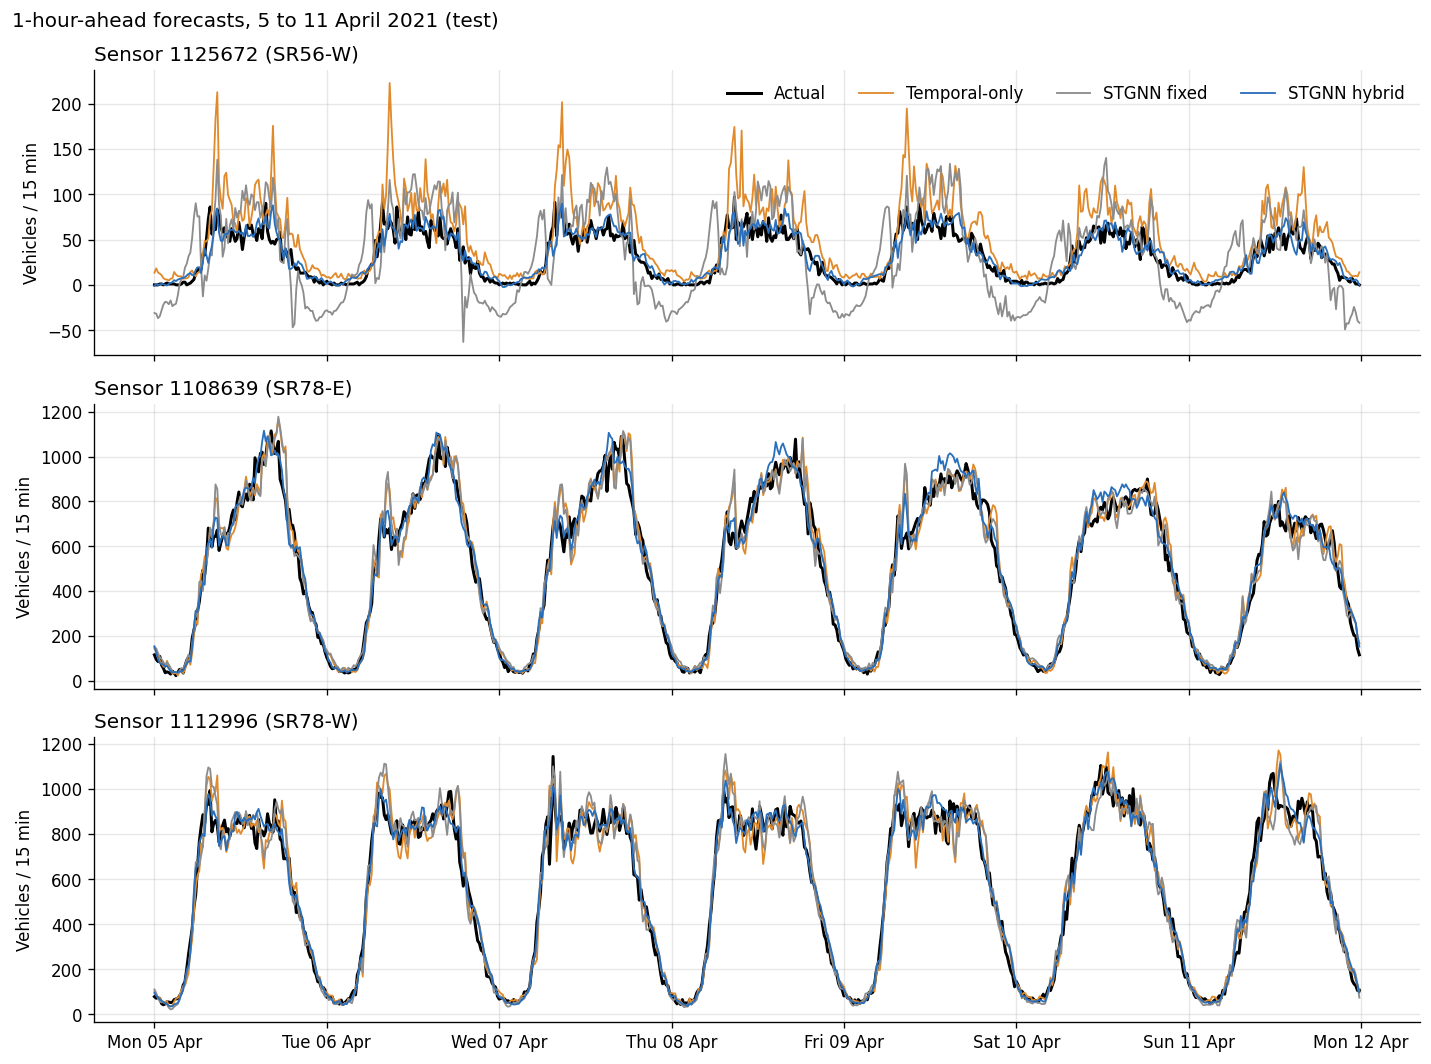
\includegraphics[width=\textwidth]{figures/q6_predictions.png}
\end{minipage}
\vspace{4pt}

\begin{itemize}[label={}]
    \item
    \begin{enumerate}[start=4]
        \item A learned graph can win because the loss picks useful links anywhere and drops unhelpful road neighbours; it can lose by overfitting or learning artefacts, and it ignores the roads that congestion actually travels along.
    \end{enumerate}
\end{itemize}

\vspace{4pt}\noindent\begin{minipage}{\textwidth}
\centering\footnotesize
\textbf{Table 3: each sensor's 10 strongest learned links compared with road edges and random pairs}\\[2pt]
\begin{tabular}{@{}lrrrr@{}}
\toprule
Sensor pairs & In road graph & Median distance & Within 5 km & Mean 2020 flow correlation \\
\midrule
Road edges & 100\% & 2.4 km & 100\% & 0.837 \\
Strongest learned links & 5.1\% & 21.4 km & 8.4\% & 0.851 \\
All pairs & 3.4\% & 23.0 km & 5.9\% & 0.824 \\
\bottomrule
\end{tabular}
\end{minipage}
\vspace{4pt}

\begin{itemize}
    \item \textbf{(c) Discussion:} \emph{Lower error does not mean the learned graph is the road network:} it beats the fixed graph by 12\% while its links are no closer than random pairs, because it is trained only to reduce the loss. \emph{A hybrid can win} because the road graph gives a reliable local prior from the start and the learned graph adds long-range links; here it kept only a small road share. \emph{A static graph is limited} because one set of weights is used all day, while the useful neighbours change: morning and evening commutes load opposite directions, congestion spreads only while a road is congested, and nights, weekends and incidents behave differently. A graph that changes with time of day or current traffic could follow this.
\end{itemize}
